\chapter{Documento de Arquitectura de Software}
\section{Introducción}
\subsection{Propósito}
El presente documento de arquitectura de software tiene como finalidad describir el sistema web Jigsaw Coding desde diferentes perspectivas, las cuales serán de gran utilidad para el desarrollo de dicho sistema. La presentación de la arquitectura del sistema será presentada haciendo uso del modelo 4+1.
\subsection{Alcance} Este documento arquitectónico aplica para describir todas las funcionalidades del sistema web a implementar. Así mismo, en este artefacto se encontrará de forma clara las 5 vistas que se describen en el modelo 4+1: Vista lógica, Vista de procesos, Vista de despliegue, Vista física y Vista de escenarios.
\begin{figure}[!h]
  \centering
  % Requires \usepackage{graphicx}
  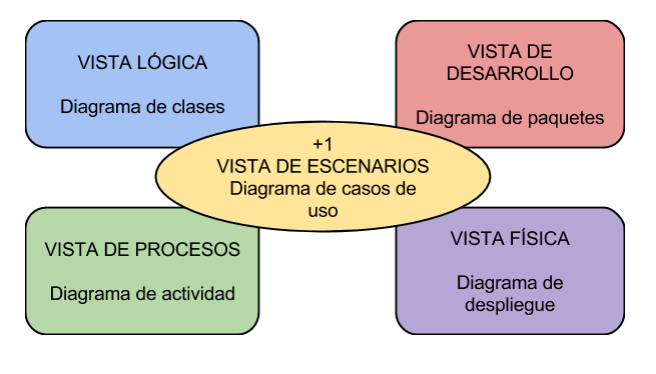
\includegraphics[scale=0.7]{figuras/sad/vista_4_mas_1.png}\\
  \caption{Modelo de arquitectura 4+1}
  \label{fig:vista_4_mas_1}
\end{figure} 
\clearpage
\section{Vista lógica}
\clearpage 
\section{Vista de procesos}
\clearpage
\section{Vista de desarrollo}
La vista de despliegue muestra el sistema desde la perspectiva del programador y se ocupa de la gestión del software a implementar. Esto es, en esta vista se describe cómo estará dividido el sistema en paquetes y las dependencias que habrá entre ellos.
\begin{figure}[!h]
  \centering
  % Requires \usepackage{graphicx}
  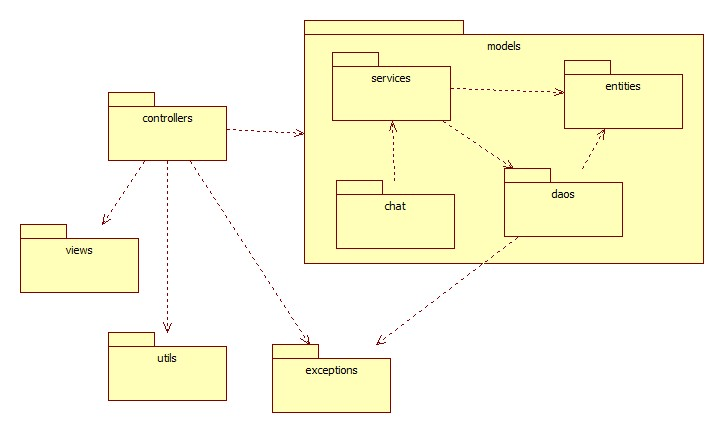
\includegraphics[scale=0.6]{figuras/sad/diagrama_de_paquetes.jpg}\\
  \caption{Diagrama de Paquetes}\label{fig:diagrama_de_paquetes}
\end{figure}
\clearpage
\section{Vista física}
\begin{figure}[!h]
  \centering
  % Requires \usepackage{graphicx}
  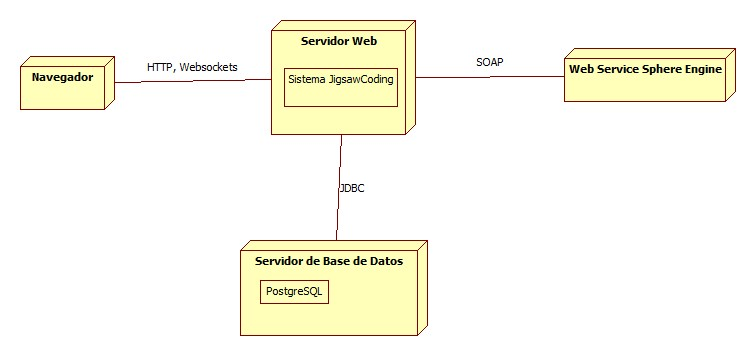
\includegraphics[scale=0.5]{figuras/sad/diagrama_de_despliegue.jpg}\\
  \caption{Diagrama de Despliegue}\label{fig:diagrama_de_despliegue}
\end{figure}
\section{Vista de escenarios}